\documentclass[a4paper]{report}
\usepackage[english]{babel}
\usepackage{amssymb}
\usepackage{amsmath}
\usepackage{graphicx}
\usepackage{float}
\usepackage{shortvrb}
\usepackage{cancel}
\usepackage[T1]{fontenc}
\usepackage{nicefrac}
\usepackage{amsfonts}
%nomenclature
\usepackage{makeidx}
\makeindex
\usepackage{nomencl}
\makenomenclature
\renewcommand{\nomname}{List of Symbols}

\usepackage{standalone} %Makes it possible to ignore other preambles of child document
\usepackage{eurosym} %Euro teken mogelijk
\usepackage{multirow} %For multiple rows togheter in one table
\usepackage{parskip} %For a small white line between paragraphs
\usepackage[protrusion=true,expansion=true]{microtype}
\usepackage{hyperref}%For automatic and URL Reference
\usepackage[titletoc]{appendix}
%Possible to change the margins
\usepackage{geometry}
\geometry{verbose,tmargin=1.9cm,bmargin=1.7cm,lmargin=1cm,rmargin=1cm}

\usepackage{subfig}

%include pdf pages
\usepackage{pdfpages}

%Small titles
\usepackage[small,compact]{titlesec}

%being able to create tables over multiple pages
\usepackage{longtable}

\makeatletter

%Change standard font size
\renewcommand\normalsize{ \@setfontsize\normalsize{11pt}{11pt}}\normalsize  
\makeatother

\usepackage{fancyhdr}
\pagestyle{fancy}
\fancyhead{}
\fancyfoot{}

%Gives text above each page
\fancyhead[CO,CE]{DSE Project}

%Page number
\fancyfoot[RO,LE]{\thepage}


\usepackage{babel}

\newcommand*{\titleDSE}{\begingroup% Three Men in a Boat
\newlength{\drop}
\setlength{\drop}{0.1\textheight}
\centering
\begin{figure}[h!]
\centering

\includegraphics[scale=0.5]{Figures/TUdelftLogo.jpg}
\end{figure}
\settowidth{\unitlength}{\LARGE AAAAAAAAAAAAAAAAAAAAAAAAAAAAAAAAAAAAAA}

\rule{\unitlength}{1.6pt}\vspace*{-\baselineskip}\vspace*{2pt}
\rule{\unitlength}{0.4pt}\\[\baselineskip]
{\LARGE Baseline Review}\\[\baselineskip]			%Main Title
{\itshape DSE All Plastic UAV}\\[0.2\baselineskip]					%subtitle
\rule{\unitlength}{0.4pt}\vspace*{-\baselineskip}\vspace{3.2pt}
\rule{\unitlength}{1.6pt}\\[\baselineskip]
\vspace*{0.1\drop}

\begin{figure}[h]
\centering
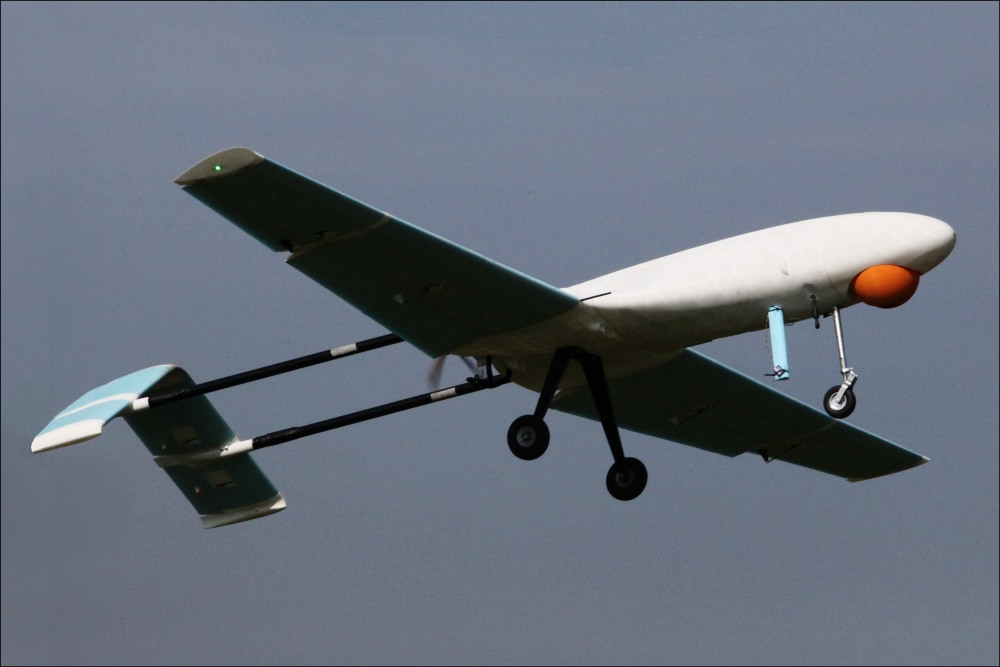
\includegraphics[width =0.75 \textwidth]{Figures/TitleImage.jpg}
\end{figure}
\vfill

\begin{table}[h]
\subfloat{
\begin{tabular}{l l}
\multicolumn{2}{l}{\textbf{Tutors}} \\
\\
Prof. dr. ir. Dingemans, T. & TU Delft\\
Ir. Melkert J. & TU Delft\\
\\
\multicolumn{2}{l}{\textbf{Coaches}}\\
\\
Ir. Bos, R. & TU Delft\\
M.Sc. Udluft H. & TU Delft
\end{tabular}
}
\hfill
\subfloat{
\begin{tabular}{r r}
\multicolumn{2}{r} {\textbf{Group members}} \\
\\
d. Heij, B. & 1507095 \\
Jeliazkov, M.K. & 4105826 \\
Kerssemakers, M.A.P. & 4005880\\
V.D. Kieboom, B. & 4114752 \\
Mooi, K. & 4020367 \\
Roelofs, M.N. & 4077407 \\
Seelen, J. & 1317547\\
v. Stralen, R. & 4019342 \\
Vendrig, P.R. & 4023838 \\
Verhoeff, C.K. & 1114344 \\
\end{tabular}
}
\end{table}

\endgroup}

%Available structures:
%Report: \part{}, \chapter{}, \section{}, \subsection{}, \subsubsection{}, \paragraph{}, \subparagraph{}

\begin{document}

\begin{titlepage}
\titleDSE
\end{titlepage}
\setcounter{page}{1} %numbering starts from here
\tableofcontents
\newpage
%\printnomenclature
\documentclass[a4paper]{report}
\usepackage[english]{babel}
\usepackage{amssymb}
\usepackage{amsmath}
\usepackage{graphicx}
\usepackage{float}
\usepackage{shortvrb}
\usepackage{cancel}
\usepackage[T1]{fontenc}
\usepackage{nicefrac}
\usepackage{amsfonts}

%nomenclature
\usepackage{makeidx}
\makeindex
\usepackage{nomencl}
\nomlabelwidth=20mm
\makenomenclature
\renewcommand{\nomname}{List of abbreviations}

\usepackage{standalone} %Makes it possible to ignore other preambles of child document
\usepackage{eurosym} %Euro teken mogelijk
\usepackage{multirow} %For multiple rows togheter in one table
\usepackage{parskip} %For a small white line between paragraphs
\usepackage[protrusion=true,expansion=true]{microtype}
\usepackage{hyperref}%For automatic and URL Reference
\usepackage[titletoc]{appendix}
%Possible to change the margins
\usepackage{geometry}
\geometry{verbose,tmargin=1.9cm,bmargin=1.7cm,lmargin=1cm,rmargin=1cm}

\usepackage{subfig}

%include pdf pages
\usepackage{pdfpages}

%being able to create tables over multiple pages
\usepackage{longtable}

\makeatletter

%Change standard font size
\renewcommand\normalsize{ \@setfontsize\normalsize{11pt}{11pt}}\normalsize  
\makeatother

\usepackage{fancyhdr}
\pagestyle{fancy}
\fancyhead{}
\fancyfoot{}

%Gives text above each page
\fancyhead[CO,CE]{DSE Project}

%Page number
\fancyfoot[RO,LE]{\thepage}


\usepackage{babel}

%Available structures:
%Report: \part{}, \chapter{}, \section{}, \subsection{}, \subsubsection{}, \paragraph{}, \subparagraph{}

\begin{document}
\chapter{Introduction (1 page)}\label{chap:Intro}
This is the Baseline Review
\end{document}
\documentclass[a4paper]{report}
\usepackage[english]{babel}
\usepackage{amssymb}
\usepackage{amsmath}
\usepackage{graphicx}
\usepackage{float}
\usepackage{shortvrb}
\usepackage{cancel}
\usepackage[T1]{fontenc}
\usepackage{nicefrac}
\usepackage{amsfonts}

%nomenclature
\usepackage{makeidx}
\makeindex
\usepackage{nomencl}
\nomlabelwidth=20mm
\makenomenclature
\renewcommand{\nomname}{List of abbreviations}

\usepackage{standalone} %Makes it possible to ignore other preambles of child document
\usepackage{eurosym} %Euro teken mogelijk
\usepackage{multirow} %For multiple rows togheter in one table
\usepackage{parskip} %For a small white line between paragraphs
\usepackage[protrusion=true,expansion=true]{microtype}
\usepackage{hyperref}%For automatic and URL Reference
\usepackage[titletoc]{appendix}
%Possible to change the margins
\usepackage{geometry}
\geometry{verbose,tmargin=1.9cm,bmargin=1.7cm,lmargin=1cm,rmargin=1cm}

\usepackage{subfig}

%include pdf pages
\usepackage{pdfpages}

%being able to create tables over multiple pages
\usepackage{longtable}

\makeatletter

%Change standard font size
\renewcommand\normalsize{ \@setfontsize\normalsize{11pt}{11pt}}\normalsize  
\makeatother

\usepackage{fancyhdr}
\pagestyle{fancy}
\fancyhead{}
\fancyfoot{}

%Gives text above each page
\fancyhead[CO,CE]{DSE Project}

%Page number
\fancyfoot[RO,LE]{\thepage}


\usepackage{babel}

%Available structures:
%Report: \part{}, \chapter{}, \section{}, \subsection{}, \subsubsection{}, \paragraph{}, \subparagraph{}

\begin{document}
\chapter{Functions and Requirements of the system (5 pages, 2 text, 3 diagrams)}\label{chap:Functions}
In this chapter the the requirements for the whole system are investigated. The requirements are found using a Requirement Discovery Tree (RDT), as is explained in section \ref{sec:RDT}. Also the functions to meet this requirements are organized. The organization of the functions is done using two separate tools, the Functional Flow Diagram (FFD) and the Functional Breakdown (FB). The FB is discussed in more detail in section \ref{sec:FB}, whereas the FFD is clarified in section \ref{sec:FFD}. 

\section{Functional Breakdown}\label{sec:FB}
The Functional Breakdown is a diagram used to find all functions the product should be able to perform. These functions are performed by a combination of minor functions. By putting all minor function under the corresponding major functions, which lead to the main function to be performed by the observation platform. The FB can be seen in figure \ref{fig:FBD}.

\begin{figure}[ht]
\includegraphics[width = \textwidth]{/Figures/FBD/FBD.png}
\label{fig:FBD}
\caption{FBD for the all plastic high altitude observation platform}
\end{figure}

\section{Functional Flow Diagram}\label{sec:FFD}
To find the required functions for different mission elements the Functional Flow Diagram is used. The FFD shows in which order different mission segments are performed, as well as what happens per segment. The flow diagram for the mission is shown in figure \ref{fig:FFD}

\begin{figure}[ht]
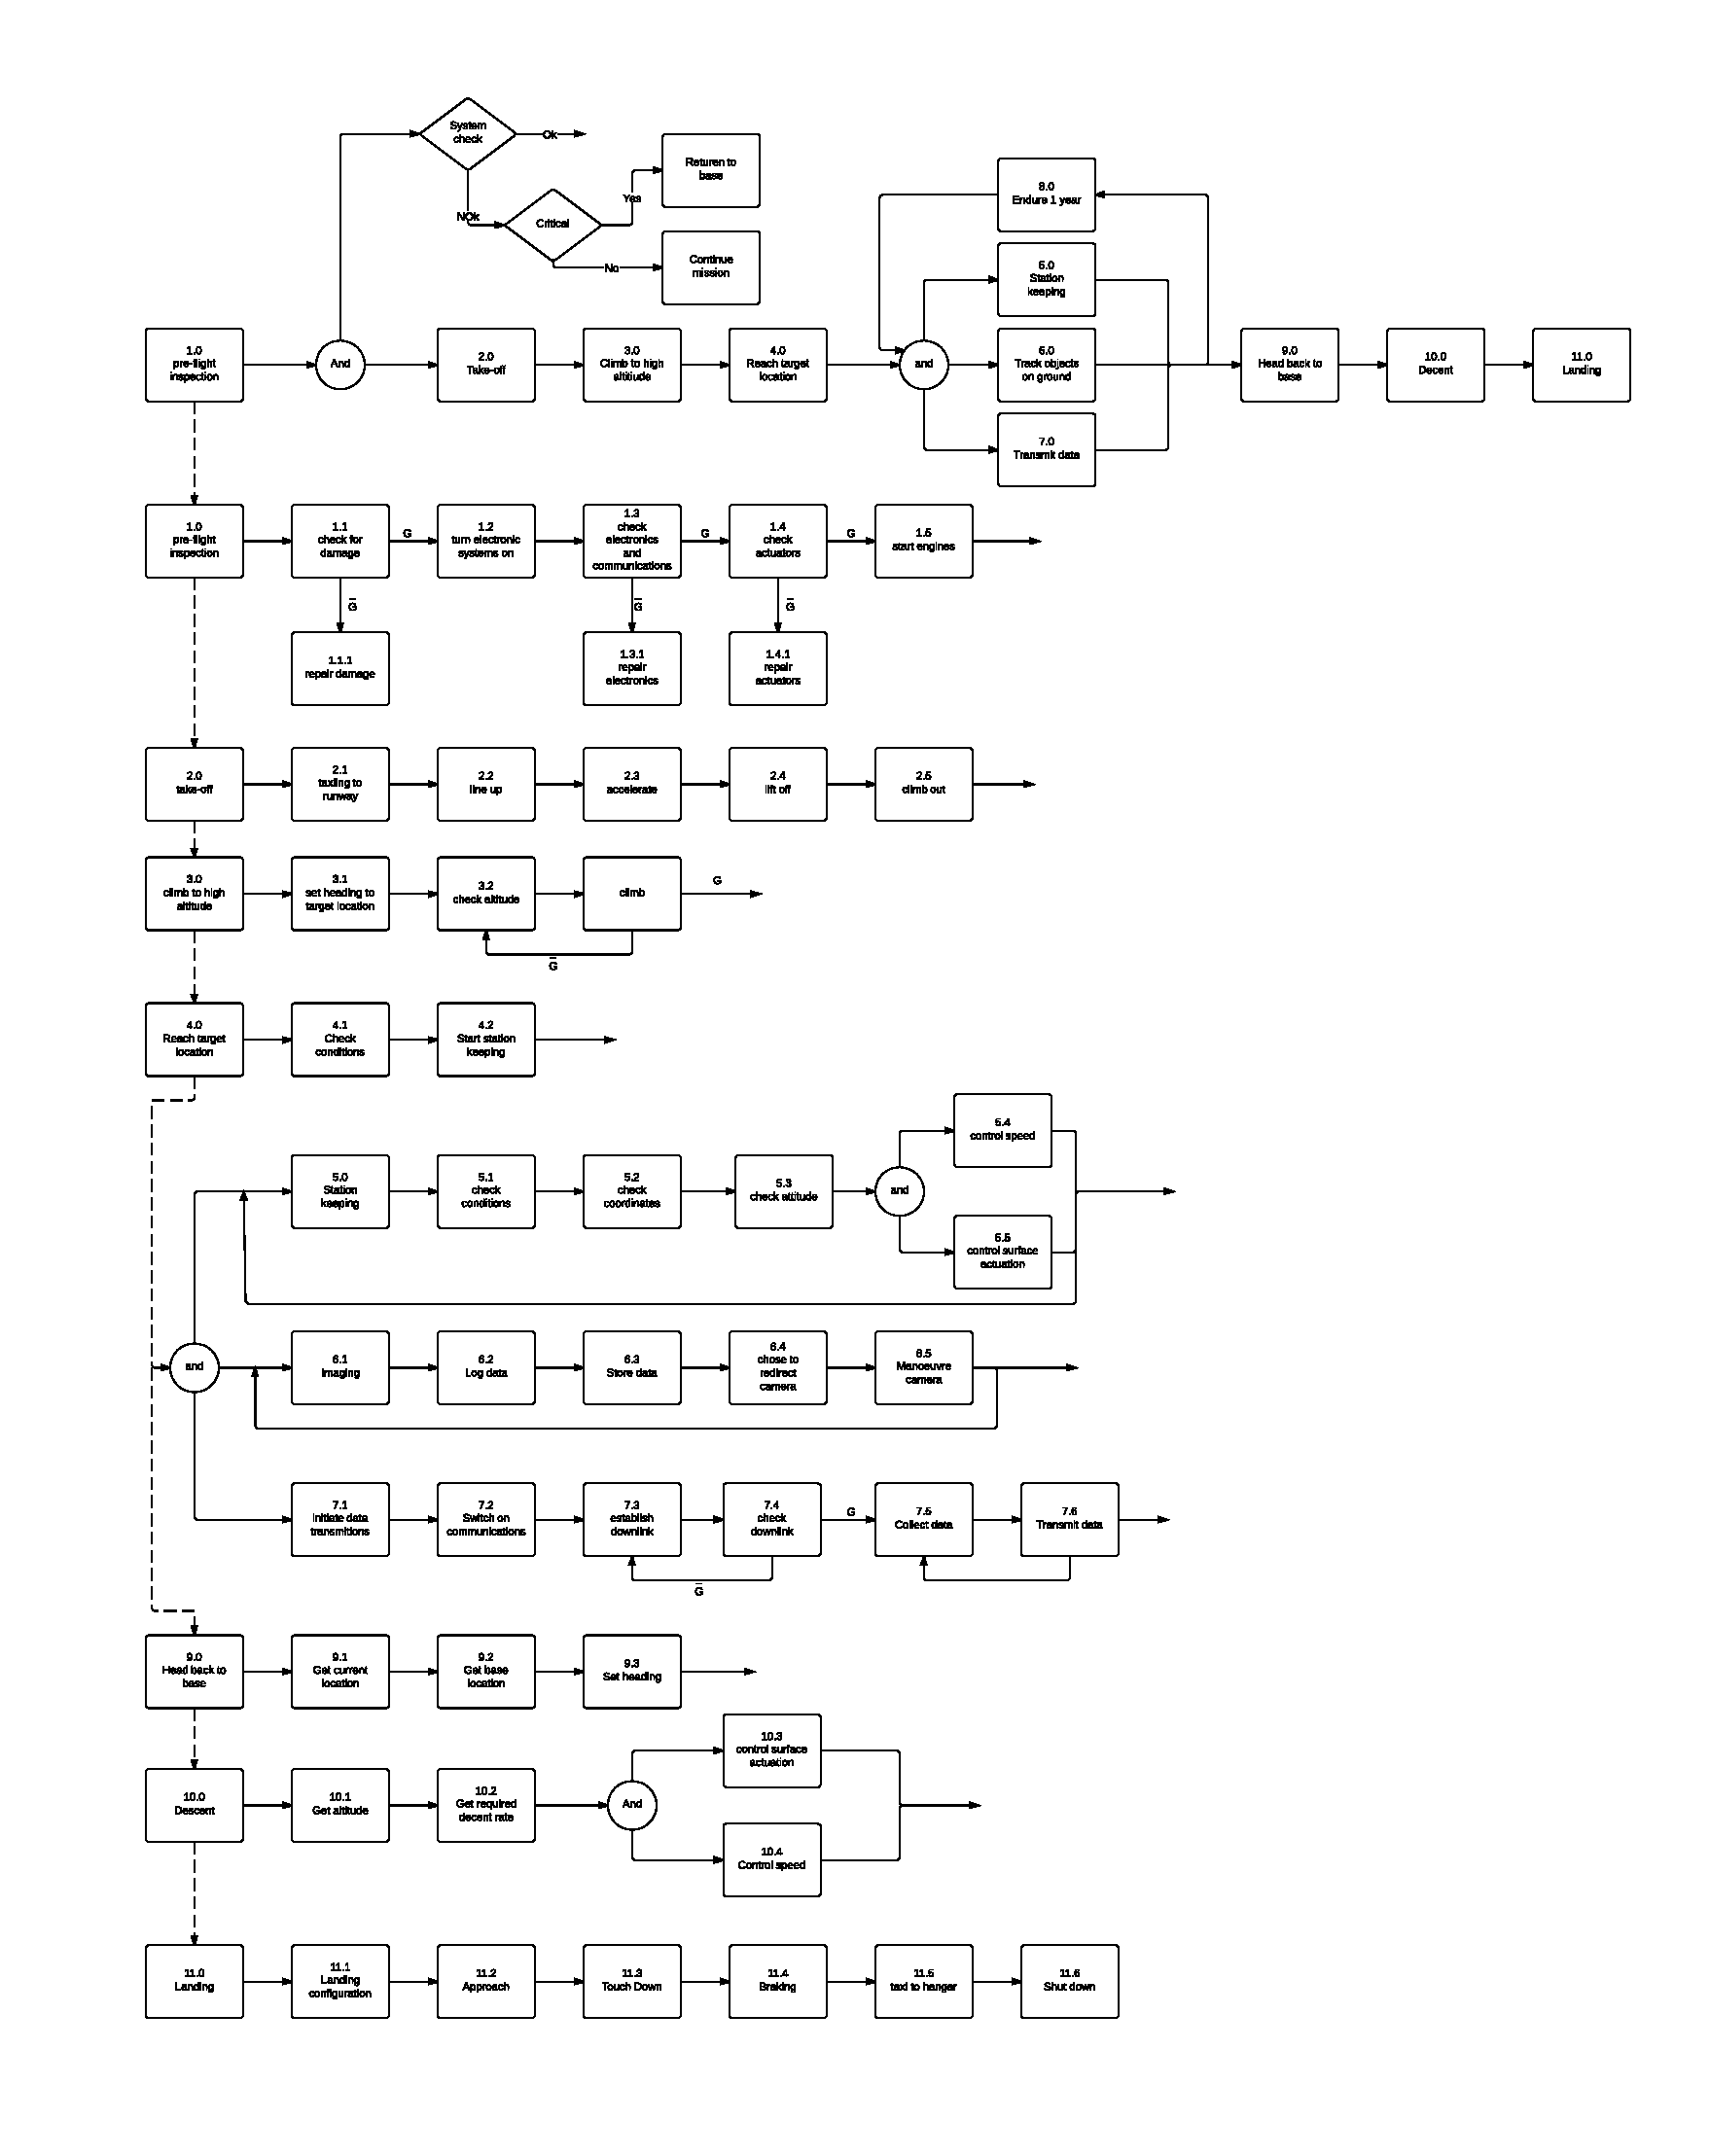
\includegraphics[width = \textwidth]{/Figures/FFD.pdf}
\label{fig:FFD}
\caption{FFD for the all plastic high altitude observation platform}
\end{figure}

\section{Requirement Discovery Tree}\label{sec:RDT}


\begin{figure}
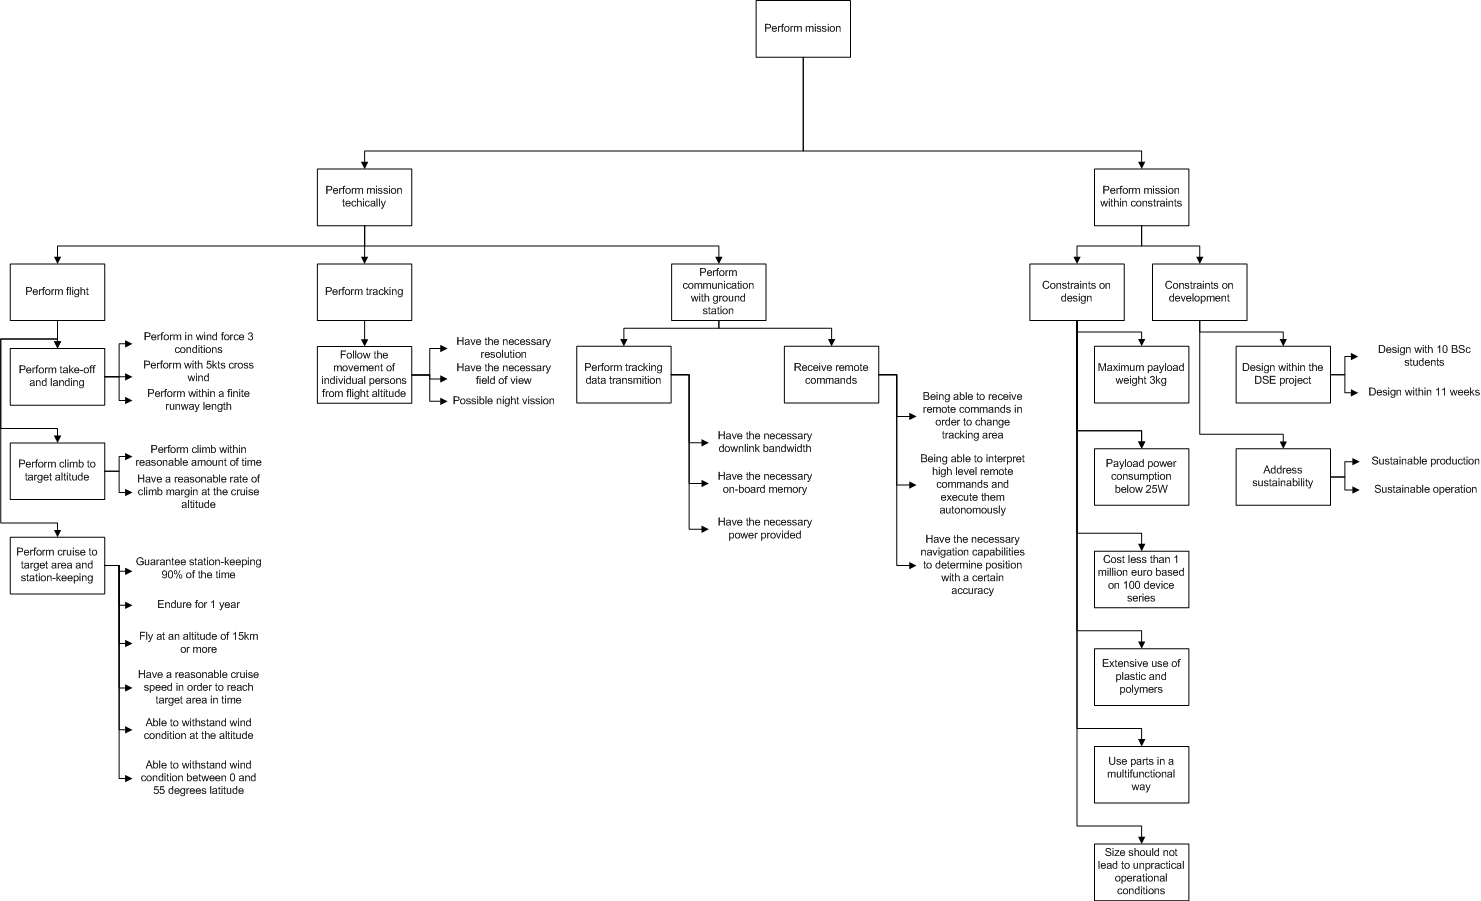
\includegraphics[width = \textwidth]{/Figures/rdt.png}
\label{fig:RDT}
\caption{RDT for the all plastic high altitude observation platform}
\end{figure}

\end{document}
\documentclass[a4paper]{report}
\usepackage[english]{babel}
\usepackage{amssymb}
\usepackage{amsmath}
\usepackage{graphicx}
\usepackage{float}
\usepackage{shortvrb}
\usepackage{cancel}
\usepackage[T1]{fontenc}
\usepackage{nicefrac}
\usepackage{amsfonts}

%nomenclature
\usepackage{makeidx}
\makeindex
\usepackage{nomencl}
\nomlabelwidth=20mm
\makenomenclature
\renewcommand{\nomname}{List of abbreviations}

\usepackage{standalone} %Makes it possible to ignore other preambles of child document
\usepackage{eurosym} %Euro teken mogelijk
\usepackage{multirow} %For multiple rows togheter in one table
\usepackage{parskip} %For a small white line between paragraphs
\usepackage[protrusion=true,expansion=true]{microtype}
\usepackage{hyperref}%For automatic and URL Reference
\usepackage[titletoc]{appendix}
%Possible to change the margins
\usepackage{geometry}
\geometry{verbose,tmargin=1.9cm,bmargin=1.7cm,lmargin=1cm,rmargin=1cm}

\usepackage{subfig}

%include pdf pages
\usepackage{pdfpages}

%being able to create tables over multiple pages
\usepackage{longtable}

\makeatletter

%Change standard font size
\renewcommand\normalsize{ \@setfontsize\normalsize{11pt}{11pt}}\normalsize  
\makeatother

\usepackage{fancyhdr}
\pagestyle{fancy}
\fancyhead{}
\fancyfoot{}

%Gives text above each page
\fancyhead[CO,CE]{DSE Project}

%Page number
\fancyfoot[RO,LE]{\thepage}


\usepackage{babel}

%Available structures:
%Report: \part{}, \chapter{}, \section{}, \subsection{}, \subsubsection{}, \paragraph{}, \subparagraph{}

\begin{document}
\chapter{Design Options (6 pages excl. DOT, is in appendix}\label{chap:DOT}
Before even coming up with several concepts or a design, it is useful to expand all potential design options.

\end{document}
\documentclass[a4paper]{report}
\usepackage[english]{babel}
\usepackage{amssymb}
\usepackage{amsmath}
\usepackage{graphicx}
\usepackage{float}
\usepackage{shortvrb}
\usepackage{cancel}
\usepackage[T1]{fontenc}
\usepackage{nicefrac}
\usepackage{amsfonts}
\usepackage{standalone} %Makes it possible to ignore other preambles of child document
\usepackage{eurosym} %Euro teken mogelijk
\usepackage{multirow} %For multiple rows togheter in one table
\usepackage{parskip} %For a small white line between paragraphs
\usepackage[protrusion=true,expansion=true]{microtype}
\usepackage{hyperref}%For automatic and URL Reference
\usepackage[titletoc]{appendix}
%Possible to change the margins
\usepackage{geometry}
\geometry{verbose,tmargin=1.9cm,bmargin=1.8cm,lmargin=2cm,rmargin=2cm}

\usepackage{subfig}

%include pdf pages
\usepackage{pdfpages}

%being able to create tables over multiple pages
\usepackage{longtable}

\makeatletter

%Change standard font size
\renewcommand\normalsize{ \@setfontsize\normalsize{11pt}{11pt}}\normalsize  
\makeatother

\usepackage{fancyhdr}
\pagestyle{fancy}
\fancyhead{}
\fancyfoot{}

%Gives text above each page
\fancyhead[CO,CE]{DSE Project}

%Page number
\fancyfoot[RO,LE]{\thepage}


\usepackage{babel}

%Available structures:
%Report: \part{}, \chapter{}, \section{}, \subsection{}, \subsubsection{}, \paragraph{}, \subparagraph{}

\begin{document}
\chapter{Resource Allocation and Budget Breakdown (3 pages)}\label{chap:RABB}

In this chapter the technical resources for the system are defined and allocated to the different necessary subsystems of the vehicle. Since the concept of the vehicle is still unknown, different general concepts will be discussed. The technical budgets that are important for this mission are the mass budget, the power budget and the link budget computing power budget. The mass budget assigns estimated percentages of the overall weight to the different parts of the vehicle. It will be a preliminary estimation to get limits on the weight of components to make sure the total weight stays within a margin of the estimated total weight. The power budgets allocates the power that is generated and can be used to the systems that require power. The computing resources budget allocates the available computing power necessary for the mission to the subsystems that require computing power. Other budgets are the height budget, the endurance budget and the dimensions budget. These depend on the concept and are first estimates on the possible heights to be flown at, maximum endurance and maximum dimensions.

The mass budget can be divided into the following components:
\begin{itemize}
\item Payload
\begin{itemize}
\item Camera
\item Lens
\item Support structure
\end{itemize}
\item Propulsion system
\item Computing & communications system
\item Power supply system
\item Electrical system
\item Structures
\begin{itemize}
\item Airframe
\item Fuselage
\item Control surfaces
\item Landing gear
\item Nacelles
\end{itemize}
\end{itemize}
\end{document}
\documentclass[a4paper]{report}
\usepackage[english]{babel}
\usepackage{amssymb}
\usepackage{amsmath}
\usepackage{graphicx}
\usepackage{float}
\usepackage{shortvrb}
\usepackage{cancel}
\usepackage[T1]{fontenc}
\usepackage{nicefrac}
\usepackage{amsfonts}

%nomenclature
\usepackage{makeidx}
\makeindex
\usepackage{nomencl}
\nomlabelwidth=20mm
\makenomenclature
\renewcommand{\nomname}{List of abbreviations}

\usepackage{standalone} %Makes it possible to ignore other preambles of child document
\usepackage{eurosym} %Euro teken mogelijk
\usepackage{multirow} %For multiple rows togheter in one table
\usepackage{parskip} %For a small white line between paragraphs
\usepackage[protrusion=true,expansion=true]{microtype}
\usepackage{hyperref}%For automatic and URL Reference
\usepackage[titletoc]{appendix}
%Possible to change the margins
\usepackage{geometry}
\geometry{verbose,tmargin=1.9cm,bmargin=1.7cm,lmargin=1cm,rmargin=1cm}

\usepackage{subfig}

%include pdf pages
\usepackage{pdfpages}

%being able to create tables over multiple pages
\usepackage{longtable}

\makeatletter

%Change standard font size
\renewcommand\normalsize{ \@setfontsize\normalsize{11pt}{11pt}}\normalsize  
\makeatother

\usepackage{fancyhdr}
\pagestyle{fancy}
\fancyhead{}
\fancyfoot{}

%Gives text above each page
\fancyhead[CO,CE]{DSE Project}

%Page number
\fancyfoot[RO,LE]{\thepage}


\usepackage{babel}

%Available structures:
%Report: \part{}, \chapter{}, \section{}, \subsection{}, \subsubsection{}, \paragraph{}, \subparagraph{}

\begin{document}
\chapter{Market analysis (4 pages)}\label{chap:MarketAnal}

\end{document}
\documentclass[a4paper]{report}
\usepackage[english]{babel}
\usepackage{amssymb}
\usepackage{amsmath}
\usepackage{graphicx}
\usepackage{float}
\usepackage{shortvrb}
\usepackage{cancel}
\usepackage[T1]{fontenc}
\usepackage{nicefrac}
\usepackage{amsfonts}

%nomenclature
\usepackage{makeidx}
\makeindex
\usepackage{nomencl}
\nomlabelwidth=20mm
\makenomenclature
\renewcommand{\nomname}{List of abbreviations}

\usepackage{standalone} %Makes it possible to ignore other preambles of child document
\usepackage{eurosym} %Euro teken mogelijk
\usepackage{multirow} %For multiple rows togheter in one table
\usepackage{parskip} %For a small white line between paragraphs
\usepackage[protrusion=true,expansion=true]{microtype}
\usepackage{hyperref}%For automatic and URL Reference
\usepackage[titletoc]{appendix}
%Possible to change the margins
\usepackage{geometry}
\geometry{verbose,tmargin=1.9cm,bmargin=1.7cm,lmargin=1cm,rmargin=1cm}

\usepackage{subfig}

%include pdf pages
\usepackage{pdfpages}

%being able to create tables over multiple pages
\usepackage{longtable}

\makeatletter

%Change standard font size
\renewcommand\normalsize{ \@setfontsize\normalsize{11pt}{11pt}}\normalsize  
\makeatother

\usepackage{fancyhdr}
\pagestyle{fancy}
\fancyhead{}
\fancyfoot{}

%Gives text above each page
\fancyhead[CO,CE]{DSE Project}

%Page number
\fancyfoot[RO,LE]{\thepage}


\usepackage{babel}

%Available structures:
%Report: \part{}, \chapter{}, \section{}, \subsection{}, \subsubsection{}, \paragraph{}, \subparagraph{}

\begin{document}
\chapter{Sustainable development (1 page)}\label{SustDev}

\end{document}



\newpage
\bibliographystyle{aiaa}
\bibliography{Bibliography/bibliography}


\begin{appendices}

\end{appendices}

\end{document}